\documentclass[12pt]{article}
\usepackage{fullpage,enumitem,amsmath,amssymb,graphicx,array}

\begin{document}

\begin{center}
{\Large Project Progress Report}

\begin{tabular}{rl}
SUNet ID: & paulmtz \\
Names: & Paul Martinez, Calvin Studebaker \\
\end{tabular}
\end{center}

\section*{Introduction}

We are interested in the process of automatically generating music playlists given a set of songs. More specifically, we would like to train an algorithm that partitions a set of songs according to some criteria that it has been trained on. After some discussion of various approaches to the problem, we will consider the specific case where we are simply trying to partition a set of songs into two distinct sets. In this case we may phrase the problem as a sort of classification algorithm, but we will explore various other potential approaches along the way.

\section*{Model}

\subsection*{Error Function}

To begin we would like to formally define the problem and the objective function we are trying to maximize. The task we would like to accomplish is to be given a set of songs $S$ and generate $K$ playlists $P_1, P_2, \ldots, P_K$ from the set $S$. These sets $P_1, \ldots, P_K$ will form a partition of the set $S$. The goal is that this partition would be similar to how a human might divide the songs up into separate playlists. To do so, we first need to define an error function between a proposed partition and a given partiion. Suppose that we are given a set $S$ and a ``correct'' partition $P = \{P_1, \ldots, P_K\}$ and our algorithm generates a partition $Q = \{Q_1, \ldots, Q_K\}$. We want to capture the difference between these sets, so we could count the number of elements that are in one set but not the other. For two sets $A$ and $B$, this can be expressed as $|(A \cup B) - (A \cap B)|$. Since the sets are unordered, different comparisions may give different counts, so we should consider the lowest possible count. Let $\pi$ be a permutation of $1, \ldots, K$. Then we can define an error function $\varepsilon$ as follows:
$$
\varepsilon(Q | P) = \min_\pi \sum_{i=1}^K |(P_i \cup Q_{\pi(i)}) - (P_i \cap Q_{\pi(i)})|
$$
To give an example, let $S = \{1, \ldots, 9\}$ and $K = 3$. Then let:
\begin{align*}
  P_1 &= \{1, 2, 3\}\\
  P_2 &= \{4, 5, 6\}\\
  P_3 &= \{7, 8, 9\}\\
  Q_1 &= \{3, 4\}\\
  Q_2 &= \{1, 2, 6\}\\
  Q_3 &= \{5, 7, 8, 9\}\\
\end{align*}
Then the optimal pairing compares $P_1$ with $Q_2$, $P_2$ with $Q_1$ and $P_3$ with $Q_3$: Then we have that $\varepsilon(Q | P) = 2 + 3 + 1 = 6$.

\subsection*{Generating Function}

Now we turn to the question of how we might generate a partition of songs. For example, we could simply produce some feature vectors for each song and then run the K-means algorithm on the feature vectors and return those as the partitions. This would produce playlists where each playlist consists of ``similar" songs, where the definition of similar is a function of the feature vectors. Alternatively consider an ``inverted'' K-means algorithm where we generate $|S| / K$ clusters, then create playlists by picking a random song from each cluster. This would create very diversifed playlists. So that we can actually train these algorithms, we can make them functions of $w$ which is in the same dimension as the feature vectors. In a K-means example, this may designate the weights of the various coordinates when calculating distance. Without any explicit representation of these functions, it is impossible to give precise algorithms for improving their performance, but we can still pose it as a general search problem and present a very rough algorithm for finding better solutions. We can try to attempt a random local-search with hill-climbing. Let $F(S; w)$ be our partition generating function and $S_1, \ldots, S_m$ be a training set of sets of songs with given partitions $P_1, \ldots, P_m$. Then we could perform the following:

\texttt{initialize w = 0}

\texttt{repeat i times or until convergence:}

\texttt{\qquad pick c random values $w_1, \ldots, w_c$ from $S_\varepsilon(w)$ (the sphere of radius $\varepsilon$ centered at w)}

\texttt{\qquad let $w_{best} = \arg \min_{w_k} \sum_{i=1}^m \varepsilon(F(S_i; w_k) | P_i)$}

\texttt{\qquad let $w = \eta w + (1 - \eta) w_{best}$ }

One could then imagine that, if given a number of partition generating functions $F_1, F_2, \ldots$, we could simply train each of them on a training set, then pick the one that had the best overall training error.

\subsection*{Classification When K = 2}

Let's consider the special case of when we are simply trying to separate the given songs into two playlists. In this case, we can simply look at the problem as a classification problem, but there are a number of subtleties involved. It would be great if we could simply combine all of individual partitions into one giant set of training examples, but we don't know in each training example which partition should be viewed as the positive examples. We need to consider each possible labelling of the examples partitions, of which there are $2^m$. We could consider each possible labelling of the individual partitions, then train a single classifier on all of them together, then pick the classifier that gave the smallest training error depending on the labelling. This too has issues however. Note that we aren't necessarily interested in a true classifier that gives either a yes-no answer, but rather interested in the relative differences between songs. If we were to use a classifier that returned a score, we could then turn that into a partitioner by simply sorting the given songs by their score, then splitting that sorted list into two (instead of dividing it at 0).

There is a still an issue that needs to be addressed. Consider the image below, where we have two training sets $S_1$ and $S_2$ and we want to train a linear classifier of the form $h(x) = w^\top x + b$ for the two sets. A linear classifier trained on $S_1$ would give the red line, and one trained on $S_2$, but if we were to train one on both sets combined, we would get something like the blue line, which does a very poor job of classifying the data. We can avoid this issue by assigning a separate intercept term to training set, so that we get a single weight vector $w$ that indicates the general axis we're comparing songs on.

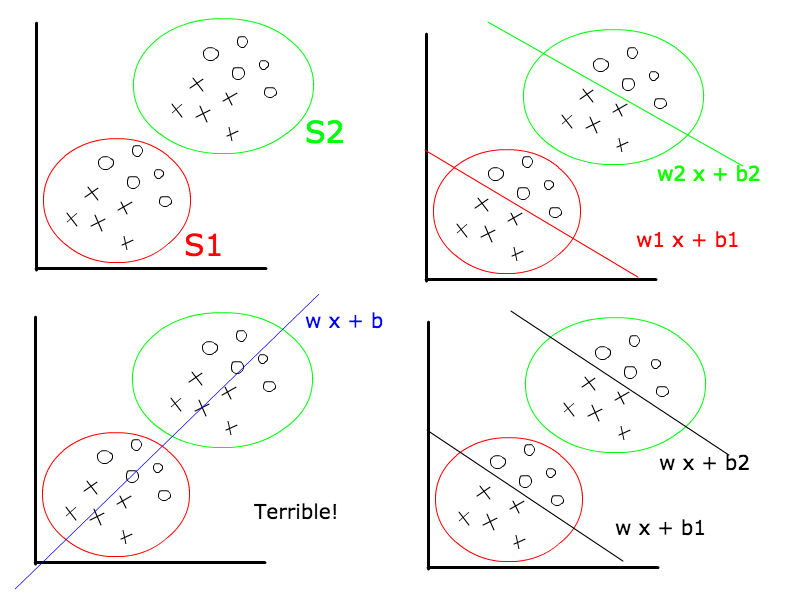
\includegraphics[scale=0.5]{interceptTerms}

\section*{Data}

We are currently pulling data from SoundCloud using their API. Some of the features regarding the songs that we have include:
\begin{enumerate}
  \item Length
  \item Artist
  \item Number of Comments
  \item Download count
  \item Playback count
  \item Like count
  \item BPM
  \item Average Volume
  \item Various text features, such as comments, tags, description, etc.
\end{enumerate}


\end{document}
